% The Journal of Risk Model Validation, revision R1 (single-column journal format).
% BLIND manuscript: the main text carries NO author name or affiliation. Author
% details live on the SEPARATE title page (title_page.tex). Author-date (APA-style)
% references, 150-200 word abstract, 4-6 keywords, 3-4 key messages of at most
% 85 characters, under 10,000 words.
%
% Sources of numbers (round 2 of R1, 2026-11-20): paper/revision-R1/round2/
% exact.json (scripts/run_round2_exact.py), ebacktest.json
% (scripts/run_round2_ebacktest.py), windows.json (scripts/run_round2_windows.py),
% exact_passrates.log; carried-over R1 figures from paper/revision-R1/
% SIMULATION-RESULTS.md and rerun-2026-11-20/. Log: paper/VERIFICATION-LOG.md.
% Earlier texts: revision-R1/main-R0.tex, main-R1-prepanel.tex, main-R1-round1.tex.
%
% Build: pdflatex -> bibtex -> pdflatex -> pdflatex  (see build.sh)

\documentclass[11pt]{article}

\usepackage[letterpaper,margin=1in]{geometry}
\usepackage{amsmath,amssymb,amsthm}
\usepackage{dsfont}
\usepackage{graphicx}
\usepackage{booktabs}
\usepackage{array}
\usepackage{float}
\usepackage[round,authoryear]{natbib}
\usepackage[font=small,labelfont=bf]{caption}
\usepackage{url}
\usepackage[hidelinks]{hyperref}

\newcolumntype{L}[1]{>{\raggedright\arraybackslash}p{#1}}
\newtheorem{remark}{Remark}

\renewcommand{\topfraction}{0.9}
\renewcommand{\bottomfraction}{0.9}
\renewcommand{\textfraction}{0.08}
\renewcommand{\floatpagefraction}{0.8}
\setcounter{topnumber}{3}
\setcounter{totalnumber}{5}

\setlength{\parindent}{0pt}
\setlength{\parskip}{6pt}
\bibliographystyle{apalike}

\begin{document}

\begin{center}
{\LARGE\bfseries The Minimum Detectable Understatement of a Passed
Value-at-Risk Backtest\par}
\vspace{8pt}
{\normalsize Submitted for blind peer review\par}
\end{center}
\vspace{4pt}

\begin{abstract}
\noindent
A value-at-risk (VaR) backtest reports pass or fail. Under independent
exceptions, a count-based panel has an exact, distribution-free minimum
detectable exception probability. The minimum detectable
understatement (MDU) of VaR follows from it through the tail quantile. The
paper tabulates the MDU of the proportion-of-failures (POF), Christoffersen and
traffic-light tests over 250 to 1,000 days at 99\% and 97.5\% coverage. Under a
strict pass rule any rejection fails a model. Under a lenient rule only too
many exceptions do. Take 250 days at 99\% and a Gaussian tail. No test of 5\%
size that reads only the exceptions detects an understatement below 13.5\% of
VaR half the time, or below 19.7\% with probability 80\%. The standard panel
nearly attains both limits. Student-$t$ tails with five degrees
of freedom raise them to 21\% and 29\%. A wrong tail makes correct models fail
far more often, while estimation error in a correct model changes the figures
little. Extra tests, including an e-backtest of expected shortfall tied to VaR,
add little unless the model updates volatility slowly. After the fact, a pass
excludes even less, but only through hindsight. The power
calculation is classical; the contribution is its tabulated inverse.
\end{abstract}

\vspace{4pt}
\noindent\textbf{Keywords:} value-at-risk, backtesting, model validation,
statistical power, minimum detectable effect, expected shortfall

\vspace{6pt}
\noindent\textbf{Key messages:}
\begin{itemize}\setlength{\itemsep}{2pt}
\item A count-based backtest detects an exception probability, not a VaR understatement.
\item One year, 5\% size: no count test detects an understatement under 13.5\% half the time.
\item At equal size, extra tests add little unless the model updates volatility slowly.
\item Reporting the minimum detectable understatement beside each pass takes four steps.
\end{itemize}
\vspace{6pt}

\noindent\fbox{\begin{minipage}{0.97\textwidth}\small
\textbf{Notation and terms.} Formulas use fractions; tables and prose use
percent, and ``points'' means percentage points. \textbf{VaR}: value-at-risk,
the loss level that the loss exceeds with probability $\alpha$ ($\alpha = 1\%$
at 99\% coverage). \textbf{ES}: expected shortfall, the mean loss on days when
the loss exceeds VaR. \textbf{Exception}: a day on which the loss exceeds the
reported VaR; $x$ counts the exceptions in $T$ days. \textbf{POF}: the
proportion-of-failures test of the exception count. \textbf{Reference}
$V^*_t$: the true conditional quantile, that is, the correct VaR.
\textbf{S0 to S4}: the reported series of Table~\ref{tab:series}; $k$ is the
number of exceptions after which S2 stops cutting VaR. \textbf{Panel}: a set
of tests that must all pass. \textbf{Strict rule}: any rejection fails the
model. \textbf{Lenient rule}: only too many exceptions fail it
(Section~\ref{sec:setup}). \textbf{Size}: the probability that a panel rejects
the reference. \textbf{Power}: the probability that it rejects an
understatement. $\mathbf{p^*_\beta}$: the exception probability at and above which
a panel rejects with probability at least $\beta$ (50\% or 80\%). $\mathbf{u^*_\beta}$ (\textbf{MDU}): the same limit
as a share of VaR. \textbf{Power envelope}: the MDU of the most powerful test
that reads only the exceptions, at the same size. \textbf{Eligible window}: one
on which the reference passes the panel (Section~\ref{sec:expost}).
\end{minipage}}

\section{Introduction}
\label{sec:intro}

Backtesting supports regulatory capital for market risk under the internal
models approach. A bank reports a value-at-risk (VaR) forecast each day. After
the fact, the supervisor counts the exceptions, the days on which the realized
loss exceeded the forecast. Three tests are standard. The
first is the proportion-of-failures (POF) test of \citet{kupiec1995}. The second
is the pair of independence and conditional coverage tests of
\citet{christoffersen1998}. The third is the traffic light of the Basel
Committee on Banking Supervision \citep{bcbs1996}, which counts exceptions over
250 days. A validator who runs these tests learns one bit: pass or fail.

How much comfort should a pass give? The direct answer is power, the
probability of rejection under a given misspecification. Power is classical.
\citet{kupiec1995} showed that it is low in samples of regulatory length. The
Basel Committee \citep{bcbs1996} tabulated the exact probability of each
exception count over 250 days when true coverage is 98, 97, 96 or 95\%.
\citet{campbell2005} simulated the power of the POF test when reported VaR is a
fixed fraction of the true VaR. These sources give the power of one test at a
few alternatives. This paper proposes no new test. It inverts power for joint
panels, compares panels at equal size against the best test available, and
states the result in the unit a validator uses. The
\textbf{minimum detectable understatement} (MDU) of a panel is the smallest
understatement of VaR that the panel rejects with a stated probability, such as
50\% or 80\%. The convention follows the minimum detectable effects of
experimental design \citep{bloom1995}. Size and power at a few alternatives
do not tell a validator what a pass rules out. The MDU does, in one number: a
small MDU means that a pass excludes all but small understatements, and a
large MDU that it excludes little.

If exceptions are independent with a common probability $p$,
the rejection probability of any count-based panel depends on $p$ alone. The
panel therefore fixes a minimum detectable exception probability that does not
depend on the loss distribution. The tail enters only when this probability is
converted into a percentage of VaR.

The paper also reports an ex post bound, the \textbf{maximum undetectable
understatement}. On a fixed window of realized losses it is the largest mean
shortfall of a reported VaR series below the reference that still passes the
panel. It has a closed form for count-based tests. The series that attains it
reads the realized losses and is rejected on every path of fresh losses. The
bound is therefore a short statement about the information in a pass: a
count-based pass says nothing about VaR on days without an exception. The MDU
is the ex ante counterpart and the main subject. For every panel tabulated
here, a constant understatement below the MDU at power $\beta$ passes with
probability above $1-\beta$. This was checked at 60 exception probabilities
below $p^*_\beta$ in every cell of Tables~\ref{tab:mdu99} and
\ref{tab:tails}(a). The check is needed because
the claim does not follow from the definition when a power curve is not
monotone.

Why would a bank understate VaR at all? Market-risk capital rises with the
reported measure, so a lower figure costs less. \citet{begley2017} find that
banks underreport trading-book risk when their equity capital is lower.
\citet{lucas2001} and \citet{daveiga2012} find that the multiplier schedule may
not deter underreporting, and \citet{cuoco2006} model reported VaR as a choice
of the bank. \citet{perignon2008} find that six large Canadian banks overstate
VaR. This paper does not claim that banks understate VaR. It measures how large
an understatement a pass would fail to exclude.

The benchmark is a constant fraction of the true VaR (series S1 below). It
needs no knowledge of future losses, and a volatility forecast scaled down by a
fixed factor produces it. The incentive is modest but not zero. In the
multiplier schedule of the Basel Framework, a constant 10\% understatement
lowers expected capital by 3.7\%. It leaves the bank in the green zone with
probability 52\%, against 89\% for a correct forecast
(Section~\ref{sec:incentive}). S1 assumes that the bank knows the true
quantile. When the reference is estimated from a correct model, the MDU changes
by at most 0.4 points. With a wrong tail the panel rejects correct models far
more often (Section~\ref{sec:estref}).

The contributions are five. First, exact MDU tables for the POF, Christoffersen
and traffic-light tests, alone and combined. They cover 250 to 1,000 days, 99\%
and 97.5\% coverage, a strict and a lenient rule, and the desk-level rule of
the revised framework. Second, a comparison of panels at an equal 5\% size against
the power envelope. The standard panel comes close to it, so differences between
pass rules are mostly differences in size. Third, measurements of what happens
when the assumptions fail: an estimated reference, a wrong tail, and clustered
exceptions. Fourth, the MDU in basis points over every rolling window of three
assets, under fitted tails. Fifth, the closed form of the ex post bound and a
four-step recipe for validators.

\section{Related work}
\label{sec:related}

\citet{kupiec1995} proposes the POF likelihood ratio (LR) test of the
unconditional exception rate and notes its low power in short samples.
\citet{christoffersen1998} adds LR tests of independence and of conditional
coverage based on the Markov transition counts of the exception sequence.
\citet{escanciano2010} show that estimation risk in the forecast model can
distort the size of these tests.
\citet{kratz2018} test exceptions at several VaR levels jointly. This test needs
forecasts at more than one level and is outside the scope of the bounds given
here.

\citet{campbell2005} reviews these tests and simulates their power against a
VaR that is systematically under-reported. Reported VaR is based on a fraction
of the true volatility, and the under-reporting ranges from 5 to 25\%. The constant understatement studied here is therefore not new, and neither is
its power curve (his Table~3 is reproduced in Appendix~\ref{app:checks}).
\citet{thiele2019} shows that tests of unconditional coverage are weaker
against underestimates of risk, and proposes one-sided Lagrange multiplier
tests. The non-monotone POF curve in Section~\ref{sec:mdu} is an instance of
this asymmetry. Exact finite-sample distributions of the Christoffersen
statistics by dynamic programming are available in the R package ExactVaRTest
\citep{exactvartest}. The dynamic program of Section~\ref{sec:exact} serves a
different purpose, the rejection probability of a joint panel under an
alternative, but the device is not new.

The traffic light of 1996 remains in the revised market risk framework
\citep{bcbsmar}. Bank-wide one-day VaR at the 99th percentile is
backtested on the most recent 250 trading days. The exception count places the
bank in a green, amber or red zone. The zone sets a multiplier of 1.50 for 0 to
4 exceptions, rising to 1.92 for 9 and 2.00 for 10 or more (MAR32.9 of the
Basel Framework). For other sample sizes the
zone boundaries come from the binomial distribution under 99\% coverage. The
amber zone begins at the smallest count whose cumulative probability is at
least 95\%, and the red zone at 99.99\% (MAR99.17). The capital measure itself is now expected shortfall (ES), the mean loss
beyond VaR, at the 97.5th percentile.

VaR is elicitable \citep{gneiting2011}: a scoring rule exists whose expected
value is smallest at the true VaR. VaR and ES are jointly elicitable
\citep{fissler2016}. \citet{nolde2017} use this to propose comparative
backtests, which score a bank's forecast against a reference forecast on every
day, not only on exception days. 
\citet{wang2025} propose e-backtesting, an anytime-valid test based on
e-values, nonnegative statistics whose expectation is at most one under the
null hypothesis. An e-backtest of ES is called an ``ES e-backtest'' below.

\section{Setup and definitions}
\label{sec:setup}

\subsection{Losses, forecasts and exceptions}

Let $\mathit{loss}_t$ be the loss of a position on day $t$, the negative of its
simple return. A VaR forecast $V_t \ge 0$ at tail probability $\alpha$ is a loss
level that the loss should exceed with probability $\alpha$. The paper uses
$\alpha = 0.01$ (99\% coverage) and $\alpha = 0.025$ (97.5\% coverage). An
exception occurs on day $t$ when $\mathit{loss}_t > V_t$; the indicator is
$e_t = \mathds{1}[\mathit{loss}_t > V_t]$. The evaluation window has $T$ days,
and $x = \sum_t e_t$ is the number of exceptions in it.

The reference forecast $V^*_t$ is the true conditional $\alpha$-quantile of the
loss given information to day $t-1$. In the model used throughout,
$\mathit{loss}_t = \sigma_t \varepsilon_t$, where $\sigma_t$ is known at the end
of day $t-1$ and the shocks $\varepsilon_t$ are independent and identically
distributed with upper quantile function $Q$. Then $V^*_t = \sigma_t
Q(\alpha)$.

\subsection{Forecaster, validator and information sets}

The \textbf{forecaster} is the bank. It reports $V_t$ each
day and, where the panel uses it, an ES forecast $S_t$. The
\textbf{validator} is the supervisor or an internal model validation unit. It
runs a fixed panel of tests on the reported series and the realized losses.


A reported series is \textbf{non-anticipating} if the value for day $t$ uses
only information available at the end of day $t-1$, including past returns and
the forecaster's own past exceptions. A series is \textbf{ex post} if it uses
the realized losses of the window on which it is tested. Only non-anticipating
series are feasible for a bank. Table~\ref{tab:series} lists the series.

\begin{table}[tbp]
\caption{Reported series studied. S0 to S3 use no future losses, but assume
that the true quantile $V^*_t$ is known.}
\label{tab:series}
\small
\centering
\begin{tabular}{lL{4.0cm}L{5.6cm}L{3.0cm}}
\toprule
Label & Name & Reported VaR on day $t$ & Information used \\
\midrule
S0 & Reference & $V^*_t$ & returns to $t-1$ \\
S1 & Constant understatement & $(1-u)V^*_t$, $u$ fixed in advance & returns to $t-1$ \\
S2 & Count-feedback understatement & $(1-u)V^*_t$ until $k$ exceptions have occurred ($k$ fixed in advance), then $V^*_t$ & returns and own exceptions to $t-1$ \\
S3 & Clustered understatement & $(1-c)V^*_t$ on high-volatility days only, or $(1-c)$ times a slowly updating volatility forecast & returns to $t-1$ \\
S4 & Exact ex post series & the closed-form solution of Section~\ref{sec:expost} & whole window \\
\bottomrule
\end{tabular}
\end{table}

\subsection{Tests, panels and pass rules}

Table~\ref{tab:tests} lists the tests. The LR tests use a 5\% significance
level. The traffic light uses the zone boundaries of the Basel
Committee: 5 and 10 at $T = 250$. For other $T$ it uses the binomial rule of
Section~\ref{sec:related}, which gives amber from 9, 12 and 15 exceptions and
red from 15, 20 and 24 at $T = 500$, 750 and 1,000. The zone rule is defined for 99\%
coverage only, so the traffic light is not used at 97.5\%.

\begin{table}[tbp]
\caption{Tests and their failure conditions under the two pass rules.}
\label{tab:tests}
\small
\centering
\begin{tabular}{L{3.6cm}L{5.5cm}L{5.5cm}}
\toprule
Test & Strict rule: fails when & Lenient rule: fails when \\
\midrule
POF test \citep{kupiec1995} & the LR test rejects (at $T = 250$ and 99\% coverage: $x = 0$ or $x \ge 7$) & it rejects and $x$ exceeds its expected value $\alpha T$ \\
Christoffersen tests \citep{christoffersen1998} & the independence or the conditional coverage test rejects & the independence test rejects, or conditional coverage rejects and $x$ exceeds $\alpha T$ \\
Traffic light \citep{bcbs1996, bcbsmar} & amber or red zone & red zone \\
ES e-backtest \citep{wang2025} & the e-process reaches 20 & the e-process reaches 20 \\
\bottomrule
\end{tabular}
\end{table}

A \textbf{panel} is a set of tests. It passes only if every test passes. The
\textbf{standard panel} combines the POF test, the Christoffersen tests and the
traffic light. Under the \textbf{strict rule} any rejection counts as failure,
including the two-sided POF rejection of too few exceptions and any exit from
the green zone. Under the \textbf{lenient rule} only evidence of too many exceptions
counts, and the traffic light fails only in the red zone. This is closer to how
a supervisor acts: the amber zone raises the multiplier but does not by itself
indicate an inaccurate model.

The \textbf{ES e-backtest} of \citet{wang2025} uses the daily e-statistic
\[
E_t = \frac{(\mathit{loss}_t - V_t)_+}{\alpha\,(S_t - V_t)}, \qquad (y)_+ = \max(y,0),
\]
where $S_t$ is stated ES. For betting fractions $\lambda_t \in [0,1/2]$ chosen
at $t-1$, the e-process $M_t = \prod_{s \le t}(1 - \lambda_s + \lambda_s E_s)$
is a nonnegative supermartingale under the null hypothesis. This means that
its expected next value does not exceed its current value. By
Ville's inequality the probability that it ever reaches 20 is at most 1/20, so
rejecting when $M_t$ reaches 20 has size at most 5\%. The
\textbf{mixture} averages the processes for the fixed fractions 0.005, 0.01,
0.02, 0.05, 0.1, 0.2, 0.35 and 0.5. The \textbf{GREM} rule (growth rate for
empirical mixture) is the adaptive default of \citet{wang2025}, which chooses each betting
fraction from past data. Unless stated otherwise, stated ES is tied to stated
VaR by the Gaussian ratio, $S_t = \kappa(\alpha) V_t$, with $\kappa(0.01) = 1.1457$.

\subsection{The two measures}

\textbf{Minimum detectable understatement (ex ante).} Fix a panel, a rule, $T$
and $\alpha$. Let $\pi(p)$ be the probability that the panel rejects when the
exceptions are independent Bernoulli draws with probability $p$. The
\textbf{minimum detectable exception probability} at power $\beta$ is
\[
p^*_\beta = \inf\{p > \alpha : \pi(p') \ge \beta \text{ for every } p' \ge p\}.
\]
The clause ``for every $p' \ge p$'' handles power curves that are not
monotone. For a loss tail with upper quantile function $Q$, the
\textbf{minimum detectable understatement} is
\[
u^*_\beta = 1 - \frac{Q(p^*_\beta)}{Q(\alpha)}.
\]
The paper reports $\beta = 0.5$ and $\beta = 0.8$. The value 0.8 is the usual
convention for minimum detectable effects \citep{bloom1995}. The MDU at
$\beta = 0.5$ is the largest constant understatement that the panel is at least
as likely to pass as to reject.

\begin{remark}
\label{prop:sep}
Let $\mathit{loss}_t = \sigma_t \varepsilon_t$ as above, with $Q$ continuous and
strictly decreasing, and let the reported VaR be $(1-u)V^*_t$. Then the
exceptions are independent Bernoulli draws with probability $p(u) =
\bar{F}\bigl((1-u)Q(\alpha)\bigr)$, where $\bar{F}$ is the upper tail of
$\varepsilon_t$. Every count-based panel rejects with probability
$\pi(p(u))$, and the panel detects the understatement $u$ with probability at
least $\beta$ at every $u' \ge u$ if and only if $u \ge u^*_\beta$.
\end{remark}

\textit{Reason.}
On day $t$ the exception is $\mathds{1}[\varepsilon_t > (1-u)Q(\alpha)]$. It
depends on $\varepsilon_t$ only, so the exceptions are independent with common
probability $p(u)$. A count-based test is a function of the exception sequence,
so its rejection probability is $\pi(p(u))$. The map $u \mapsto p(u)$ is
continuous and strictly increasing, and its inverse is $p \mapsto 1 -
Q(p)/Q(\alpha)$, which carries $p^*_\beta$ to $u^*_\beta$.

The panel, the rule, $T$ and $\alpha$ fix $p^*_\beta$; the tail fixes only the
conversion to a percentage of VaR. The ES e-backtest reads the size of each
breach, so it is not covered by the remark and is studied by simulation.

\textbf{Equal size and the power envelope.} Panels with different sizes are
not directly comparable. For a comparison at a common size, each component test
is given its $p$-value. The panel rejects when the smallest $p$-value is below
a common critical value. When the smallest $p$-value equals the critical value,
the panel rejects with a probability chosen so that the size is exactly 5\%.
This is randomization at the boundary, the standard device for equal sizes of
discrete tests \citep[Chapter~3]{lehmann2005}. Under independent
Bernoulli($p$) exceptions the count $x$ is sufficient and the likelihood ratio
increases in $x$. The randomized one-sided binomial test is therefore uniformly
most powerful against $p > \alpha$ \citep[Section~3.4]{lehmann2005}. No test
that reads only the exception sequence has more power at the same size,
including the Christoffersen tests and the duration-based test of
\citet{christoffersen2004}. Its MDU is called the
\textbf{power envelope}.

\textbf{Maximum undetectable understatement (ex post).} Fix a panel and a
window of realized losses on which the reference passes the panel. Such a
window is called \textbf{eligible}. The ex post bound $\Delta^\star$ is the
largest mean understatement $T^{-1}\sum_t (V^*_t - V_t)$ over all reported
series with $0 \le V_t \le V^*_t$ that pass the panel. It is a property of the
panel and the window, not a strategy.

\textbf{Units.} Both measures are given as a percentage of VaR and in basis
points (bp) of notional. On a notional of USD 1 billion (US dollars), 1 bp is
USD~100,000.

\section{Method, data and simulation design}
\label{sec:method}

\subsection{Exact rejection probabilities}
\label{sec:exact}

The POF test depends on the exception sequence through $x$. The traffic light
depends on $x$ when the window is the full sample. The Christoffersen tests
depend on $x$, the number of adjacent exception pairs, and whether the first
and the last day are exceptions. A dynamic program over these four statistics
gives their exact joint distribution under independent Bernoulli($p$)
exceptions for any $T$. Each pass or fail flag comes from the test code, applied to a synthetic
sequence with the given statistics. The rejection probability $\pi(p)$ is then
a finite sum. The limit $p^*_\beta$ is located on a grid of 301 values of $p$
and refined by root search.

Three checks support the exact values (Appendix~\ref{app:checks}). At $T = 250$
they reproduce every value of a separate implementation, for example a size of
20.24\% for the strict standard panel. Monte Carlo estimates on 20,000 paths
agree with them within 1.75 standard errors in all ten cells checked. The
exact POF power at the under-reporting levels of \citet{campbell2005} agrees
with his simulated values within 1.6 standard errors at 5 to 20\%, when only
too many exceptions count. At 25\% the exact value is 89.4\% against his
79.7\%, and the gap is unexplained (Appendix~\ref{app:checks}).

\subsection{Data and reference forecast}
\label{sec:data}

Real data serve the conversion of the MDU into basis points and the ex post
bound. The data are daily closing prices adjusted for splits and
dividends for 2015 to 2024, from Yahoo Finance through the yfinance Python
package. Three positions are used: Apple Inc.\ common stock
(ticker AAPL), the SPDR S\&P~500 exchange-traded fund (ETF) Trust (ticker SPY)
and Bitcoin priced in US dollars (ticker BTC-USD). The cache holds 2,514, 2,514 and 3,651 daily returns. Bitcoin trades every calendar day, so 250 returns span about eight months. Each position is held at constant notional, so its profit and loss is
hypothetical: the change in value of a portfolio held fixed over the day.

The reference forecast on real data is $z_\alpha \hat\sigma_t$, with
$z_{0.01} = 2.3263$ the Gaussian quantile and $\hat\sigma_t$ a causal
volatility forecast, which uses only data up to the previous day. For the first 500 days $\hat\sigma_t$ is the exponentially
weighted moving average (EWMA) of squared returns with decay 0.94, started from
the sample variance of the first 5\% of returns. This start uses data inside
the first windows. After that, a
generalized autoregressive conditional heteroscedasticity model of order (1,1),
GARCH(1,1), is refitted every 25 days on an expanding window. Windows of 250
days start every 25 days, and the most recent 250 days form one more window.
This gives 92 windows for AAPL and SPY and 138 for BTC-USD. Every result below
uses all of them, and no window is selected. Three alternative references are
also run on every window with enough history. The first is the Student-$t$
quantile times the same volatility. The second is filtered historical
simulation (FHS), which multiplies the volatility by the empirical quantile of
the previous 500 standardized losses. The third is historical simulation (HS),
the empirical quantile of the previous 250 losses.

\subsection{Simulation design}
\label{sec:simdesign}

\textbf{E-backtest.} With a reference equal to the true conditional quantile
and a constant understatement, each e-value and each exception depends only on
the shock of the day. Independent Gaussian shocks therefore give the same
rejection law as a GARCH path. Each path has 1,000 days, and rejection by horizon $T$
means a crossing before day $T$. The understatement runs from 0 to 45\%. Every
level uses the same simulated shocks (common random numbers), so the curves are
comparable. The mixture uses 10,000 paths and the GREM rule 5,000
paths of 500 days. The MDU is read from the simulated curve by linear
interpolation. Its standard error (the binomial standard error at the crossing divided by the
slope) is at most 0.14 points.

\textbf{Estimated reference.} Paths of 1,250 days are drawn from a GARCH(1,1)
model with the parameters fitted to each asset, with Gaussian or Student-$t$
shocks. The validator estimates the reference from the path, with the Gaussian
quantile, and the last 250 days form the window. Three estimators are
used: the rolling GARCH(1,1) of Section~\ref{sec:data}, refitted every 25 days
on the 1,000 or more preceding days; EWMA with decay 0.94; and HS on the
previous 250 days. The reported VaR is $(1-u)$ times the estimated reference.
Each case uses 5,000 paths.

\textbf{Clustered understatement.} Paths are drawn from the same GARCH models
with Gaussian shocks and the true reference. In two variants the forecaster
cuts VaR by a fraction $c$ only on days whose volatility, known at $t-1$, is
above the median or the 80th percentile of its previous 250 values. In a third
variant the forecaster reports $(1-c)$ times a Gaussian EWMA forecast with
decay 0.99, a slowly updating model. All three series are non-anticipating, and
their exceptions cluster in volatile spells. Each case uses 10,000 paths, at
$T = 250$ and 1,000. Rejection is compared with the exact rejection of a
constant understatement with the same mean understatement.

\textbf{Fresh losses for the ex post series.} On each eligible window the ex
post series and the observed volatility $V^*_t/z_\alpha$ are kept and the shocks
are redrawn, 500 paths per window. The shocks are Gaussian or Student-$t$, with
degrees of freedom fitted by maximum likelihood: 4.97 for AAPL, 6.71 for SPY and
3.16 for BTC-USD.

\section{Results: the minimum detectable understatement}
\label{sec:mdu}

\subsection{Panels and pass rules at 99\% coverage}

Table~\ref{tab:mdu99} reports the exact size, $p^*_\beta$ and the Gaussian MDU
at 99\% coverage for every window length, panel and rule.
Figure~\ref{fig:curves} shows the exact power curves.

\begin{table}[tbp]
\caption{Exact detection limits at 99\% coverage, Gaussian tail, in percent:
size, minimum detectable exception probability $p^*_\beta$ and MDU $u^*_\beta$
at power $\beta = 50\%$ and $80\%$.}
\label{tab:mdu99}
\footnotesize
\centering
\setlength{\tabcolsep}{3pt}
\begin{tabular}{rl rrrrr rrrrr}
\toprule
 & & \multicolumn{5}{c}{Strict rule} & \multicolumn{5}{c}{Lenient rule} \\
\cmidrule(lr){3-7}\cmidrule(lr){8-12}
$T$ & Panel & Size & $p^*_{0.5}$ & $u^*_{0.5}$ & $p^*_{0.8}$ & $u^*_{0.8}$ & Size & $p^*_{0.5}$ & $u^*_{0.5}$ & $p^*_{0.8}$ & $u^*_{0.8}$ \\
\midrule
250 & POF & 9.5 & 2.66 & 16.9 & 3.61 & 22.7 & 1.4 & 2.66 & 16.9 & 3.61 & 22.7 \\
 & Traffic light & 10.8 & 1.87 & 10.5 & 2.67 & 17.0 & $<$0.1 & 3.86 & 24.0 & 4.97 & 29.2 \\
 & POF + Christ. & 10.9 & 2.64 & 16.8 & 3.59 & 22.6 & 2.8 & 2.64 & 16.8 & 3.60 & 22.6 \\
 & Standard panel & 20.2 & 1.81 & 10.0 & 2.64 & 16.8 & 2.8 & 2.64 & 16.8 & 3.60 & 22.6 \\
\addlinespace
500 & POF & 7.1 & 1.93 & 11.1 & 2.49 & 15.7 & 3.1 & 1.93 & 11.1 & 2.49 & 15.7 \\
 & Traffic light & 6.7 & 1.73 & 9.2 & 2.27 & 14.0 & $<$0.1 & 2.93 & 18.7 & 3.61 & 22.7 \\
 & POF + Christ. & 8.5 & 1.92 & 11.0 & 2.49 & 15.7 & 4.5 & 1.93 & 11.0 & 2.49 & 15.7 \\
 & Standard panel & 12.1 & 1.72 & 9.1 & 2.26 & 13.9 & 4.5 & 1.93 & 11.0 & 2.49 & 15.7 \\
\addlinespace
750 & POF & 4.1 & 1.82 & 10.1 & 2.26 & 13.9 & 2.1 & 1.82 & 10.1 & 2.26 & 13.9 \\
 & Traffic light & 7.8 & 1.56 & 7.3 & 1.97 & 11.4 & $<$0.1 & 2.62 & 16.6 & 3.14 & 20.0 \\
 & POF + Christ. & 6.1 & 1.81 & 10.0 & 2.26 & 13.9 & 4.1 & 1.81 & 10.0 & 2.26 & 13.9 \\
 & Standard panel & 11.8 & 1.55 & 7.2 & 1.96 & 11.4 & 4.1 & 1.81 & 10.0 & 2.26 & 13.9 \\
\addlinespace
1,000 & POF & 5.5 & 1.67 & 8.5 & 2.03 & 12.0 & 2.6 & 1.67 & 8.5 & 2.03 & 12.0 \\
 & Traffic light & 8.2 & 1.47 & 6.3 & 1.81 & 9.9 & $<$0.1 & 2.37 & 14.7 & 2.79 & 17.8 \\
 & POF + Christ. & 7.2 & 1.66 & 8.4 & 2.02 & 11.9 & 4.3 & 1.66 & 8.4 & 2.02 & 11.9 \\
 & Standard panel & 12.7 & 1.46 & 6.3 & 1.81 & 9.9 & 4.3 & 1.66 & 8.4 & 2.02 & 11.9
\\
\bottomrule
\end{tabular}
\\[2pt]
\footnotesize Traffic light: fails outside the green zone (strict) or in the
red zone (lenient). Christ.: Christoffersen.
\end{table}

\begin{figure}[tbp]
\centering
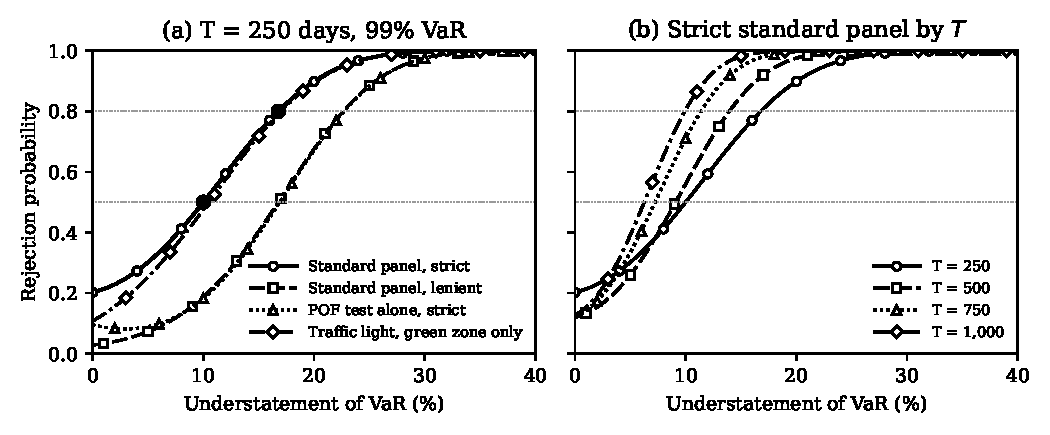
\includegraphics[width=\textwidth]{../figures/fig_mdu_curves.pdf}
\caption{Exact rejection probability of a constant understatement of VaR at
99\% coverage, Gaussian tail. Dots in (a) mark the MDU of the strict standard
panel at 50\% and 80\% power. In (a) the strict standard panel and the traffic
light alone are close, as are the lenient standard panel and the POF test
alone; Table~\ref{tab:mdu99} gives their MDUs.}
\label{fig:curves}
\end{figure}

\textbf{One year.} With 250 days, the strict standard panel rejects a correct
forecast 20.2\% of the time. Its MDU is 10.0\% of VaR at 50\% power and 16.8\%
at 80\% power. A 10\% understatement corresponds to an exception probability of
1.81\%. Under the lenient rule the size falls to
2.8\%, and the MDU rises to 16.8\% and 22.6\%.

\textbf{What each test adds at nominal size.} The strict standard panel owes
its power to the green-zone rule. The traffic light alone, failing outside the
green zone, has an MDU of 10.5\% and 17.0\%, close to the full panel. The POF
test alone has 16.9\% and 22.7\%. Added to the POF test, the Christoffersen
tests lower the Gaussian MDU by at most 0.3 points at any window length, under
either rule and at either coverage level. Under the fattest tail computed
(Student-$t$ with three degrees of freedom) they lower it by at most 0.5
points. At equal size the effect differs, as the next paragraph shows. Under
the lenient rule the traffic light adds nothing at $T = 250$, since the POF
test already rejects at 7 exceptions. The POF curve is not monotone. A 5\%
understatement is rejected 8.9\% of the time, less often than the correct
forecast (9.5\%), because the two-sided test also rejects zero exceptions
\citep[see also][]{thiele2019}.

\textbf{Window length.} Longer windows help, but slowly. With 1,000 days the
strict standard panel has an MDU of 6.3\% and 9.9\%, and the lenient panel
8.4\% and 11.9\%. Four years of data thus lower the MDU of one year by 37 to
50\%. The size of the strict panel falls from 20.2\% to 12.7\%.

\textbf{Equal size.} The comparisons above mix sizes from under 0.1\% to 20.2\%,
so a lower MDU partly reflects a higher size. Table~\ref{tab:size} recalibrates
every panel to an exact 5\% size, as defined in Section~\ref{sec:setup}, and
gives the power envelope. With 250 days at 99\%, no test that reads only the
exception sequence and has 5\% size detects an understatement below 13.5\%
half the time, or below 19.7\% with probability 80\%. The traffic light and
the one-sided POF test attain this envelope, and the standard panel comes
within 0.4 points. The two-sided POF test, alone or with the Christoffersen
tests, lies 3.0 to 3.4 points above it, because part of its size goes to
rejecting too few exceptions. The Christoffersen tests raise the one-sided POF
figure by 0.8 points (14.3\% and 20.5\% against 13.5\% and 19.7\%). Under
independent exceptions they spend size without adding power. At 1,000 days
they also raise the two-sided POF figure, by 0.5 points. At its own size of
20.2\% the envelope is 7.6\% and 14.6\%, 2.4 and 2.2 points below the strict
standard panel. The ranking of pass rules above is therefore largely a ranking
of sizes.

\begin{table}[tbp]
\caption{MDU in percent at an exact 5\% size, 99\% coverage, Gaussian tail; $u^*_{0.5}$ / $u^*_{0.8}$.}
\label{tab:size}
\small
\centering
\begin{tabular}{lrrr}
\toprule
Test or panel at 5\% size & $T = 250$ & 500 & 1,000 \\
\midrule
Power envelope (one-sided POF; traffic light) & 13.5 / 19.7 & 10.1 / 14.9 & 7.4 / 10.9 \\
POF, two-sided & 16.9 / 22.7 & 12.9 / 17.3 & 8.9 / 12.4 \\
POF + Christoffersen, two-sided & 16.9 / 22.7 & 12.8 / 17.3 & 9.4 / 12.9 \\
POF + Christoffersen, one-sided & 14.3 / 20.5 & 11.0 / 15.7 & 8.4 / 11.9 \\
Standard panel, two-sided & 13.9 / 20.0 & 11.1 / 15.7 & 8.1 / 11.7 \\
\bottomrule
\end{tabular}
\\[2pt]
\footnotesize One-sided: rejection for too few exceptions is ignored. Each panel rejects when its smallest component $p$-value is below a common critical value, randomized at the boundary. Student-$t$ envelope at $T = 250$: 20.6 / 28.7 (5 degrees of freedom) and 25.6 / 34.9 (3.16).
\end{table}

\subsection{Coverage level and tail shape}

Table~\ref{tab:tails} gives the MDU at 97.5\% coverage and the effect of the
tail. At 97.5\% the POF and Christoffersen tests reach 80\% power at an
understatement of 19.9\% with 250 days and 10.9\% with 1,000 days, Gaussian
tail. At equal $T$ and power these figures lie between those of the strict and
the lenient standard panel at 99\% (Table~\ref{tab:mdu99}).

\textbf{Desk-level rule.} The revised framework also backtests each trading
desk. A desk moves to the standardized approach if it has more than 12
exceptions at the 99th percentile or 30 at the 97.5th percentile in the most
recent 12 months \citep[MAR32.19]{bcbsmar}. If both VaR levels are cut by the
same fraction, each day falls in one of three classes: loss below both VaR
levels, between them, or above the 99th percentile level. The two counts are
then trinomial, and the rejection probability is exact. Over 250 days the rule has a
size below 0.001\% and an MDU of 29.5\% and 34.3\% under a Gaussian
tail, and 40.4\% and 45.5\% under the Student-$t$ fit of AAPL. It removes
grossly inaccurate desks and does not detect moderate understatement.

\begin{table}[tbp]
\caption{MDU in percent at 50\% / 80\% power by coverage level, window length and tail.}
\label{tab:tails}
\small
\centering
\setlength{\tabcolsep}{4pt}
\begin{tabular}{llrrrr}
\toprule
\multicolumn{6}{l}{\textit{(a) 97.5\% coverage, Gaussian tail; $u^*_{0.5}$ / $u^*_{0.8}$}} \\
Panel & Rule (size at $T=250$, \%) & $T = 250$ & 500 & 750 & 1,000 \\
\midrule
POF & strict (7.4) & 14.3 / 20.1 & 10.3 / 14.6 & 8.8 / 12.4 & 8.0 / 11.2 \\
POF + Christ. & strict (9.1) & 14.1 / 19.9 & 10.1 / 14.5 & 8.6 / 12.3 & 7.7 / 10.9 \\
POF + Christ. & lenient (4.1) & 14.1 / 19.9 & 10.2 / 14.5 & 8.6 / 12.3 & 7.7 / 10.9
\\
\bottomrule
\end{tabular}

\vspace{8pt}
\begin{tabular}{lrrrr}
\toprule
\multicolumn{5}{l}{\textit{(b) 99\% coverage, $T = 250$, standard panel; measured against the true quantile of each tail}} \\
Tail & Strict $u^*_{0.5}$ & Strict $u^*_{0.8}$ & Lenient $u^*_{0.5}$ & Lenient $u^*_{0.8}$ \\
\midrule
Gaussian & 10.0 & 16.8 & 16.8 & 22.6 \\
Student-$t$, $\nu = 6.71$ (SPY fit) & 14.0 & 22.7 & 22.7 & 29.7 \\
Student-$t$, $\nu = 4.97$ (AAPL fit) & 15.7 & 25.0 & 25.0 & 32.4 \\
Student-$t$, $\nu = 5$ & 15.6 & 25.0 & 25.0 & 32.4 \\
Student-$t$, $\nu = 3.16$ (BTC-USD fit) & 19.7 & 30.6 & 30.6 & 38.9 \\
Student-$t$, $\nu = 3$ & 20.3 & 31.5 & 31.5 & 39.9
\\
\bottomrule
\end{tabular}
\\[2pt]
\footnotesize At 97.5\% the size of each panel at $T = 500$ to 1,000 is between 4.2\% and 8.0\%.
\end{table}

The tail matters as much as the pass rule. A fat tail places a given exception
probability further below the true quantile. With five degrees of freedom the
strict MDU of the standard panel is 15.6\% and 25.0\% (15.7\% and 25.0\% for
the AAPL fit); with three it is 20.3\% and 31.5\%. For the lenient rule and
$\nu = 3$ the MDU at 80\% power is 39.9\%. These are the panel's own MDUs, at
its own size of 20.2\%. At a 5\% size the envelope under five degrees of
freedom is 20.6\% and 28.7\% (Table~\ref{tab:size}).
All these figures assume that the reference is the true quantile of the fat
tail (Section~\ref{sec:estref} relaxes this).

\subsection{The ES e-backtest}

Table~\ref{tab:ebt} reports the MDU of the ES e-backtest by simulation, with ES
tied to VaR. The e-backtest alone is less powerful than the POF test at every
horizon. With 1,000 days the mixture has an MDU of 11.2\% and 14.6\%, against
8.5\% and 12.0\% for the two-sided POF test alone (Table~\ref{tab:mdu99}). The
e-backtest also has the lower size, 1.9\% against 5.5\%, so part of this gap is
size. The adaptive GREM rule is weaker than the mixture, with a size below 1\%. Adding the e-backtest to the strict standard panel lowers its MDU by
less than 0.2 points. Under the lenient rule, which the e-backtest cannot
loosen, it lowers the MDU by less than 0.9 points at both power levels and raises the
size from 2.8\% to 3.9\%.

\begin{table}[tbp]
\caption{MDU of the ES e-backtest and of panels that include it, Monte Carlo, Gaussian tail. Size and MDU in percent; 10,000 paths (mixture and panels) or 5,000 (GREM).}
\label{tab:ebt}
\small
\centering
\begin{tabular}{llrrr}
\toprule
Coverage, $T$ & Test or panel & Size & $u^*_{0.5}$ & $u^*_{0.8}$ \\
\midrule
99\%, 250 & E-backtest, mixture & 1.5 & 19.1 & 24.6 \\
99\%, 1,000 & E-backtest, mixture & 1.9 & 11.2 & 14.6 \\
99\%, 250 & E-backtest, GREM & 0.6 & 20.7 & 26.3 \\
\addlinespace
99\%, 250 & Standard panel, strict & 19.9 & 9.9 & 16.7 \\
99\%, 250 & Standard panel + e-backtest, strict & 20.6 & 9.8 & 16.6 \\
99\%, 250 & Standard panel, lenient & 2.8 & 16.7 & 22.6 \\
99\%, 250 & Standard panel + e-backtest, lenient & 3.9 & 15.9 & 21.8 \\
\addlinespace
97.5\%, 250 & E-backtest, mixture & 1.7 & 17.5 & 22.7 \\
97.5\%, 250 & POF + Christoffersen, strict & 8.9 & 14.1 & 19.8 \\
97.5\%, 250 & POF + Christoffersen + e-backtest, strict & 10.1 & 13.4 & 19.2 \\
\bottomrule
\end{tabular}
\\[2pt]
\footnotesize Standard errors of $u^*$ are at most 0.14 points. The count-test rows reproduce the exact values of Tables~\ref{tab:mdu99} and \ref{tab:tails} within 0.3 points.
\end{table}

The e-backtest tests ES, and here ES is cut
in proportion to VaR, so it has power. If stated ES is held at the reference
level while VaR is cut by 20\%, the mixture rejects only 6.6\% of the time.
Stated ES is then not too low, so its null hypothesis holds. The
results therefore say little about ES models in general. The rows at 97.5\% use
the regulatory ES level; the others use 99\%. An ES forecast whose tail beyond
VaR is wrong is not studied.

\subsection{All rolling windows: basis points and observed pass rates}

Table~\ref{tab:bps} converts the MDU of the standard panel into basis points
over all 92, 92 and 138 rolling windows. The conversion multiplies $u^*_\beta$
by the mean true VaR of each window. Under the Gaussian tail this is the mean
reference VaR. Under the Student-$t$ tail fitted to each asset, the true VaR is
the reference VaR times $Q_t(\alpha)/z_\alpha$, which is 1.12, 1.09 and 1.14
for AAPL, SPY and BTC-USD. Here $Q_t$ is the Student-$t$ quantile function and $z_\alpha$ the Gaussian
quantile, and $u^*_\beta$ is the Student-$t$ value of Table~\ref{tab:tails}(b).
On the median window of AAPL, SPY and BTC-USD the MDU of the strict standard
panel at 50\% power is then 67, 32 and 178~bp. Under a Gaussian tail it is 38,
21 and 80~bp. The Gaussian conversion understates the BTC-USD figure by more
than half.

\begin{table}[tbp]
\caption{MDU of the standard panel in basis points of notional over all rolling
windows; $T = 250$, 99\%. Median.}
\label{tab:bps}
\small
\centering
\setlength{\tabcolsep}{4pt}
\begin{tabular}{llrr}
\toprule
Asset (windows) & Tail & Strict, $\beta = 0.5$ & Strict, $\beta = 0.8$ \\
\midrule
AAPL (92) & Student-$t$ & 67.1 & 107.1 \\
 & Gaussian & 38.2 & 64.1 \\
SPY (92) & Student-$t$ & 31.6 & 51.0 \\
 & Gaussian & 20.6 & 34.6 \\
BTC-USD (138) & Student-$t$ & 178.2 & 277.4 \\
 & Gaussian & 79.8 & 133.8 \\
\bottomrule
\end{tabular}
\\[2pt]
\footnotesize Student-$t$ degrees of freedom 4.97, 6.71 and 3.16, fitted on the full sample.
\end{table}

Table~\ref{tab:passrate} applies a constant understatement to the causal
reference on every window and records how often the standard panel passes.
Windows overlap, so the rates are descriptive. In panel (a), the Gaussian
GARCH reference passes the strict panel on 34 to 64\% of windows, against 80\%
for a correctly specified forecast. On the 10, 10 and 14 non-overlapping
windows (not tabulated) its strict pass rate is 70\%, 40\% and 50\%, with
binomial standard errors of 13 and 11 points around 80\%. On these windows,
rates as low as those of SPY and BTC-USD have probabilities of 0.7\% and
1.2\% under a correct reference, whose exact pass probability is 79.8\%. The
shortfall is therefore not sampling noise. Panel (b) points to the tail as its main
source. With the fitted Student-$t$ quantile the strict pass rate at $u = 0$
rises to 50 to 74\%, and with FHS to 76 to 85\%. With FHS a 10\% understatement
passes on 58 to 76\% of windows. This exceeds the Gaussian exact value of 50\%,
as the fat-tail rows of Table~\ref{tab:tails}(b) predict.

\begin{table}[tbp]
\caption{Share of rolling windows (percent) on which a constant understatement
$u$ (percent) of a causal reference passes the standard panel; $T = 250$,
99\%. ``Exact'' gives the pass probability of a correctly specified
reference.}
\label{tab:passrate}
\small
\centering
\begin{tabular}{lrrrrr}
\toprule
\multicolumn{6}{l}{\textit{(a) Gaussian GARCH reference, strict rule}} \\
Asset & $u = 0$ & $u = 5$ & $u = 10$ & $u = 20$ & $u = 30$ \\
\midrule
AAPL & 64 & 45 & 17 & 8 & 1 \\
SPY & 34 & 28 & 22 & 10 & 4 \\
BTC-USD & 54 & 45 & 36 & 13 & 1 \\
Exact, correct reference & 80 & 70 & 50 & 10 & $<1$ \\
\bottomrule
\end{tabular}

\vspace{8pt}
\begin{tabular}{lrrr}
\toprule
\multicolumn{4}{l}{\textit{(b) Strict rule, other references; pass rate at $u = 0$ / $u = 10$}} \\
Reference & AAPL & SPY & BTC-USD \\
\midrule
Gaussian GARCH, as in (a) & 64 / 17 & 34 / 22 & 54 / 36 \\
Student-$t$ GARCH & 74 / 64 & 50 / 34 & 72 / 60 \\
Filtered historical simulation & 82 / 67 & 85 / 76 & 76 / 58 \\
Historical simulation & 62 / 55 & 40 / 37 & 69 / 43 \\
\bottomrule
\end{tabular}
\\[2pt]
\footnotesize Windows with enough history: 92, 92, 138 (Gaussian and Student-$t$), 72, 72, 118 (FHS), 82, 82, 128 (HS). The Student-$t$ degrees of freedom are fitted on the full sample, so that reference is not fully causal.
\end{table}

\subsection{Estimated and misspecified references}
\label{sec:estref}

Table~\ref{tab:estref} repeats the exact calculation with a reference that the
validator estimates, on simulated paths of each asset. First, estimation error
alone matters little when the model is right. With Gaussian shocks and a GARCH(1,1) reference estimated on four or more years, the
size is within 1.2 points and the MDU of both rules within 0.4 points of the
exact values. Second, misspecification matters a great deal. With
Student-$t$ shocks the Gaussian GARCH reference averages 87 to 91\% of the
true quantile, and the strict panel rejects it 35 to 41\% of the time. The
faster EWMA and the HS reference raise the size further, to between 26 and
64\% under the strict rule. The panel cannot tell this apart from
understatement \citep{escanciano2010}. Under the lenient rule the size is 3 to
33\%. 

\begin{table}[tbp]
\caption{Size and MDU of the standard panel when the validator estimates the
reference; $T = 250$, 99\%, 5,000 simulated paths per cell. Percent; range over
the three assets.}
\label{tab:estref}
\small
\centering
\setlength{\tabcolsep}{3pt}
\begin{tabular}{llrrrrrr}
\toprule
 & & \multicolumn{3}{c}{Strict rule} & \multicolumn{3}{c}{Lenient rule} \\
Simulated shocks & Reference & Size & $u^*_{0.5}$ & $u^*_{0.8}$ & Size & $u^*_{0.5}$ & $u^*_{0.8}$ \\
\midrule
\multicolumn{2}{l}{Exact, correctly specified} & 20.2 & 10.0 & 16.8 & 2.8 & 16.8 & 22.6 \\
Gaussian & GARCH & 20--21 & 9.6--9.7 & 16.7--16.9 & 3 & 16.5--16.6 & 22.5--22.8 \\
Gaussian & EWMA & 26--34 & 4.3--6.4 & 11.9--13.5 & 6--11 & 12.5--13.7 & 18.9--19.8 \\
Gaussian & HS & 45--61 & $0^{a}$--2.3 & 15.3--17.6 & 19--33 & 10.2--12.7 & 22.8--28.6 \\
Student-$t$ & GARCH & 35--41 & 4.3--5.4 & 15.0--19.5 & 10--14 & 15.0--17.9 & 22.8--29.5 \\
Student-$t$ & EWMA & 54--64 & $0^{a}$ & 7.4--8.5 & 20--28 & 8.8--9.5 & 17.6--19.1 \\
Student-$t$ & HS & 42--49 & 1.4--4.8 & 19.1--27.8 & 16--22 & 16.6--20.8 & 29.7--39.4 \\
\bottomrule
\end{tabular}
\\[2pt]
\footnotesize The reference uses the Gaussian quantile; $u^*$ is a percentage of the estimated reference. $^{a}$ The size exceeds 50\%, so the panel rejects the reference more often than not and the MDU at 50\% power is set to 0. Standard errors of the size are at most 0.7 points. Values for each asset are in the repository (Appendix~\ref{app:repro}).
\end{table}

\subsection{Clustered understatement}
\label{sec:cluster}

Under a constant understatement the exceptions are independent, so the
Christoffersen tests can only add size. Table~\ref{tab:cluster} reports the
series S3, which cuts VaR only on high-volatility days, with the MDU stated as
the mean understatement. First, a concentrated cut is easier to detect for a
given mean. With the cut on days above the 80th percentile of recent
volatility, the POF test detects a mean understatement of 9.0 to 9.5\% half
the time at $T = 250$. For a constant cut the figure is 16.9\%. The
exception probability rises faster than in proportion to the cut. The cut
applies on 21 to 22\% of days, not exactly 20\%, because the threshold is a
trailing percentile. Second, the clustering
is mild. The first-order autocorrelation of the exceptions is 0.04 to 0.05
(Table~\ref{tab:cluster}). The Christoffersen tests lower the MDU of the POF
test by at most 1.0 point at $T = 250$ and 0.2 points at $T = 1{,}000$.

\begin{table}[tbp]
\caption{MDU in percent of non-anticipating understatements whose exceptions
cluster, as mean understatement; strict rule, 99\%, Gaussian GARCH paths. Range
over the three assets, 10,000 paths per cell.}
\label{tab:cluster}
\footnotesize
\centering
\setlength{\tabcolsep}{2.5pt}
\begin{tabular}{rlrccc}
\toprule
$T$ & Cut on days & Lag-1 & POF & POF + Christ. & Standard panel \\
\midrule
250 & All (exact) & 0 & 16.9 / 22.7 & 16.8 / 22.6 & 10.0 / 16.8 \\
 & Above median & 0.04 & 13.1--13.3 / 17.5--19.3 & 12.9--13.1 / 17.3--19.0 & 8.2--8.4 / 13.4--14.7 \\
 & Above 80th pct. & 0.04--0.05 & 9.0--9.5 / 11.9--15.8 & 8.6--9.2 / 11.5--14.8 & 5.9--6.2 / 9.2--12.0 \\
\addlinespace
1,000 & All (exact) & 0 & 8.5 / 12.0 & 8.4 / 11.9 & 6.3 / 9.9 \\
 & Above median & 0.04 & 7.2--7.3 / 9.8--9.9 & 7.1--7.2 / 9.8 & 5.4--5.5 / 8.3--8.4 \\
 & Above 80th pct. & 0.04--0.05 & 5.4--5.7 / 6.9--7.6 & 5.2--5.5 / 6.8--7.5 & 4.2--4.4 / 6.0--6.5 \\
\bottomrule
\end{tabular}
\\[2pt]
\footnotesize Entries are $u^*_{0.5}$ / $u^*_{0.8}$; Christ.: Christoffersen; All: the constant understatement. Cut on days with volatility above the median or the 80th percentile of the previous 250 days. Lag-1: first-order autocorrelation coefficient (not a percentage) of the daily exception indicator, measured on simulated paths in which VaR is cut by 40\% on the affected days.
\end{table}

A slowly updating model clusters its exceptions after volatility rises.
Table~\ref{tab:slow} reports a Gaussian EWMA forecast with decay 0.99 and no
cut. On average it states VaR 4 to 17\% above the true quantile. The strict POF
test still rejects it 14 to 30\% of the time at $T = 250$ and 13 to 37\% at
$T = 1{,}000$, against 9.5\% and 5.5\% for a correct forecast. The Christoffersen tests add 5 to 9
points at $T = 250$ and 10 to 19 points at $T = 1{,}000$. The independence
tests therefore earn their place against slow models, not against a constant
or volatility-timed cut.

\begin{table}[tbp]
\caption{Strict rejection, in percent, of a slowly updating forecast (Gaussian
EWMA with decay 0.99, no cut); 99\% coverage, Gaussian GARCH paths, 10,000
paths per cell.}
\label{tab:slow}
\small
\centering
\begin{tabular}{rlrrr}
\toprule
$T$ & Asset & VaR above true quantile & POF rejects & POF + Christ. rejects \\
\midrule
250 & AAPL & 4.1 & 14.1 & 19.1 \\
 & SPY & 7.6 & 14.1 & 23.5 \\
 & BTC-USD & 16.7 & 30.2 & 35.1 \\
 & Correct forecast, exact & 0.0 & 9.5 & 10.9 \\
\addlinespace
1,000 & AAPL & 4.2 & 12.8 & 22.8 \\
 & SPY & 7.7 & 19.8 & 38.4 \\
 & BTC-USD & 16.0 & 36.7 & 48.5 \\
 & Correct forecast, exact & 0.0 & 5.5 & 7.2
\\
\bottomrule
\end{tabular}
\\[2pt]
\footnotesize Christ.: Christoffersen tests. The last row of each block is the
exact rejection of a correct forecast.
\end{table}

\subsection{Adaptive understatement and the multiplier schedule}
\label{sec:incentive}

\textbf{Count feedback.} The series S2 cuts VaR by a fraction $u$ until $k$
exceptions have occurred, and then reports the reference. It was simulated on
5,000 Gaussian GARCH paths per setting (AAPL parameters, true reference), with $k \in \{2,3,4\}$ and $u$ from 5\% to 50\%.
Table~\ref{tab:countfb} gives selected settings. With $k = 4$ and $u = 20\%$ the
mean understatement is 10.1\% and the strict standard panel rejects 68.5\% of
the time, against 50.3\% for a constant understatement of the same mean. With
$k = 2$ and $u = 5\%$ the rejection rate equals that of the reference on the
same paths. No setting with a
rejection rate of 50\% or less understates by more than 7.6\%. Count feedback
thus does not raise the MDU at 50\% power, but it can hide a small
understatement. The ES e-backtest, tied to VaR, rejects heavy cuts more often
than the strict standard panel (98.2\% against 92.2\% at $k = 4$ and
$u = 50\%$). It rejects light cuts less often (7.6\% against 40.9\% at
$k = 4$ and $u = 10\%$).

\begin{table}[tbp]
\caption{Count-feedback understatement S2 under the strict standard panel,
selected settings, in percent; $T = 250$, 99\%, 5,000 Gaussian GARCH paths
(AAPL parameters).}
\label{tab:countfb}
\small
\centering
\setlength{\tabcolsep}{4pt}
\begin{tabular}{rrrrrr}
\toprule
$k$ & Cut $u$ & Mean understatement & S2 rejected & Same-mean constant rejected & ES e-backtest rejected \\
\midrule
2 & 5 & 2.7 & 20.5 & 24.1 & 2.5 \\
3 & 20 & 7.6 & 49.0 & 39.5 & 19.5 \\
4 & 10 & 7.5 & 40.9 & 39.1 & 7.6 \\
4 & 20 & 10.1 & 68.5 & 50.3 & 27.7 \\
4 & 50 & 6.6 & 92.2 & 35.5 & 98.2
\\
\bottomrule
\end{tabular}
\\[2pt]
\footnotesize The reference is rejected on 20.5\% of the same paths. Same-mean
constant: exact rejection of a constant understatement equal to the mean
understatement of S2.
\end{table}

\textbf{Expected capital, an illustration.} In the revised framework the
requirement is the larger of the latest ES-based measure and the multiplier
times its 60-day average \citep[MAR33.41--33.42]{bcbsmar}. The illustration
assumes that the multiplied average binds, that the measure is cut in the same
proportion $u$ as backtested VaR, and that the multiplier follows the exception
count of one 250-day window (MAR32.9). Under a Gaussian tail the expected
multiplier of a correct forecast is 1.525. A 10\% understatement raises it to
1.633 and a 20\% understatement to 1.836. The expected capital factor $(1-u)\,
E[m(x_u)]/E[m(x_0)]$ is then 0.974 at $u = 5\%$, 0.963 at 10\%, 0.963 at 20\%
and 0.947 at 25\%. Between $u = 8\%$ and 21\% the rise in the expected
multiplier offsets the cut almost exactly, and the factor stays between 0.962
and 0.966. Under a Student-$t$ tail
with five degrees of freedom the factor is 0.931 at $u = 10\%$. The multiplier
schedule thus removes most, but not all, of the expected saving. A 10\%
understatement saves 3.7\% of capital in expectation, and it moves the bank
out of the green zone with probability 48\%, against 11\% for a correct
forecast. Other supervisory responses are ignored. The result points the same
way as
\citet{lucas2001} and \citet{daveiga2012}.

\section{Remark: what a pass cannot exclude after the fact}
\label{sec:expost}

For a fixed exception vector $e$, the largest
understatement on each day is $V_t = 0$ if $e_t = 1$ and $V_t =
\max(\mathit{loss}_t, 0)$ if $e_t = 0$. Day $t$ can be an exception only if
$\mathit{loss}_t > 0$, and must be one if $\mathit{loss}_t > V^*_t$. With
$T = 250$ the POF test and the traffic light bound only $x$, by $\bar{x} = 4$
for the strict standard panel. The optimum concedes every day with
$\mathit{loss}_t > V^*_t$ and then the largest remaining positive losses, up to
$\bar{x}$ days in total. With $e^\star$ the resulting exception vector,
\[
\Delta^\star = \frac{1}{T}\sum_{t=1}^{T} V^*_t \;-\; \frac{1}{T}\sum_{t\,:\,e^\star_t = 0} \max(\mathit{loss}_t, 0).
\]
If the optimum fails the Christoffersen tests, a repaired series gives a lower
bound. The construction uses the realized losses, so it is ex post by design.

Table~\ref{tab:expost} reports $\Delta^\star$ under the strict standard panel.
The bound is defined only on eligible windows, where the reference passes: 59,
31 and 75 of the 92, 92 and 138 windows, a selected subset. On the
152 windows where the optimum passes every test, $\Delta^\star$ is exact and
equals 83 to 93\% of the mean reference VaR. On the other 13 the repaired lower
bound lies in the same range. The exact series states zero VaR on 46 to 63\%
of days. Applied to fresh losses on each eligible window, under both shock
laws, it was rejected on every path under both rules, with 90.5 to 111.1
exceptions on average against 2.5 expected. Comparative backtests based on consistent scores \citep{nolde2017} do read the
size of VaR on days without an exception.

\begin{table}[tbp]
\caption{Ex post bound under the strict standard panel on every eligible
window.}
\label{tab:expost}
\small
\centering
\setlength{\tabcolsep}{4pt}
\begin{tabular}{lrrr}
\toprule
Asset & Eligible & $\Delta^\star$, bp, & $\Delta^\star$ / mean $V^*$, \\
 & (exact + bound) & median (IQR) & range, \% \\
\midrule
AAPL & 59 of 92 (51 + 8) & 315.9 (287.6--355.1) & 83--92 \\
SPY & 31 of 92 (26 + 5) & 167.4 (138.7--177.4) & 85--93 \\
BTC-USD & 75 of 138 (75 + 0) & 648.9 (601.2--786.9) & 87--93 \\
\bottomrule
\end{tabular}
\\[2pt]
\footnotesize Exact: windows where the optimum passes every test. Bound: windows with a repaired lower bound. IQR: interquartile range.
\end{table}

\section{A recipe for validators, and limitations}
\label{sec:recipe}

\subsection{Recipe}

A validator can report the MDU beside each pass in four steps.
\begin{enumerate}\setlength{\itemsep}{2pt}
\item Record $T$, $\alpha$, the tests applied and the pass rule actually used,
including how the amber zone is treated, and the size of that panel.
\item Read $p^*_{0.5}$ and $p^*_{0.8}$ from Table~\ref{tab:mdu99} (99\%
coverage), or compute them with the accompanying code. Tables~\ref{tab:size}
and \ref{tab:tails} give only $u^*$, not $p^*$. To compare panels, use the
equal-size values of Table~\ref{tab:size}.
\item Convert with the tail fitted to the profit and loss, $u^*_\beta = 1 -
Q(p^*_\beta)/Q(\alpha)$, and give the Gaussian value beside it. Then check the
reference. The exact figure holds for a reference whose tail is right, and an
estimated GARCH reference changes it little. If the model assumes a thinner
tail than the data, or uses a fast EWMA or HS estimator, the panel rejects a
correct model far more often than its size (Table~\ref{tab:estref}). Then
report the simulated figure for the estimator used.
\item Write beside the pass: ``this backtest would have detected a constant
understatement of $u^*_{0.8}$ or more with probability 80\%''. State that smaller
understatements are not excluded, and give the figure in basis points of the
current VaR.
\end{enumerate}
For the strict standard panel with one year at 99\%, the sentence reads
``16.8\% or more'' under a Gaussian tail and ``25.0\% or more'' with five
degrees of freedom. For the median AAPL window under its fitted tail this is
107~bp. A validator who wants a 10\% understatement detected with probability 80\%
under the strict standard panel needs about 1,000 days of data.

\subsection{Limitations}

The exact calculation assumes independent exceptions and a reference whose
tail is right. A wrong tail or a fast estimator raises the rejection rate of a
correct model, and the panel cannot separate this from understatement. The MDU
is defined for a constant understatement. The clustered and count-feedback
series are the only other non-anticipating strategies examined. The positions
are single assets with hypothetical profit and loss, not trading desks or
portfolios. The e-backtest results assume ES tied to VaR.

\section{Conclusion}
\label{sec:conclusion}

A count-based backtest detects an exception probability, not an
understatement. Under independent exceptions this probability is exact and
distribution-free, and the tail converts it into a percentage of VaR. Take one
year at 99\%, a 5\% size and a Gaussian tail. No test that reads only the
exceptions detects an understatement below 13.5\% half the time, or below
19.7\% with probability 80\%. Five
degrees of freedom raise these limits to 20.6\% and 28.7\%. The standard
panel nearly attains the envelope at equal size, so the pass rule matters
mainly through size. At its own size of 20.2\% the strict standard panel has an MDU of
10.0\% and 16.8\% under a Gaussian tail, and 15.6\% and 25.0\% with five
degrees of freedom. Against a constant or volatility-timed
understatement, extra tests add little. Against a slowly updating model the
independence tests add more. The exact figures survive estimation error in a correct model, but not a
wrong tail.

After the fact, a pass excludes even less. The ex post bound is 83 to 93\% of
mean VaR on every eligible window, but the series that attains it uses the
realized losses and is rejected on every path of fresh losses. The figure
describes the information in a pass, not a strategy.

Future work can extend the MDU to multilevel and comparative backtests
\citep{kratz2018, nolde2017} and to portfolio-level profit and loss.

\section*{Declarations}

\textbf{Declarations of Interest.} The author reports no conflicts of interest.
The author alone is responsible for the content and writing of the paper.

\textbf{Use of artificial intelligence.} AI tools (Claude, Anthropic) assisted with code,
literature checks and language editing. The research question, design, analysis
and conclusions are the author's own, and the author takes full responsibility
for the content.

\appendix

\section{Reproducibility}
\label{app:repro}

Every number in the paper comes from the accompanying code, held in a
repository whose address is on the separate title page. Separate scripts produce the exact limits, the checks and
Figure~\ref{fig:curves}; the equal-size values, desk-level rule and capital
factors; the e-backtest rows; the rolling-window results; the estimated-reference
and clustered simulations; and the count-feedback series. A last script writes
the tables from the saved output. Random numbers come from the NumPy seed
sequence $(5424, e, \ldots)$, where $e$ indexes the experiment. The repository lists the command for each table.

\section{Validation checks}
\label{app:checks}

Table~\ref{tab:checks} lists the checks behind the statements of exactness.
Table~\ref{tab:campbell} compares the exact POF power with Table~3 of
\citet{campbell2005}. His design draws one year of 255 days with known
volatility, so the exceptions are independent and the exact calculation applies.

\begin{table}[H]
\caption{Validation checks.}
\label{tab:checks}
\small
\centering
\begin{tabular}{L{9.0cm}L{5.4cm}}
\toprule
Check & Result \\
\midrule
Dynamic program: probabilities sum to one; count marginal is binomial & both within $10^{-12}$ \\
Pass flags against the test code, random sequences & 300 of 300 equal \\
Exact values at $T = 250$ against a separate implementation & 10 of 10 equal \\
Exact against Monte Carlo (20,000 paths) & 10 cells, within 1.75 standard errors \\
Size-adjusted panels against the envelope (840 points) & never above it \\
Desk-level rule against Monte Carlo (40,000 paths) & within 2.1 standard errors \\
Closed form for $\Delta^\star$ against integer programming & equal on 152 exact windows \\
$\Delta^\star$ recomputed without the constraint $V_t \le V^*_t$ of Section~\ref{sec:setup} & higher by at most 4.4~bp on the 165 eligible windows \\
\bottomrule
\end{tabular}
\end{table}

\begin{table}[H]
\caption{POF power under under-reporting of VaR: exact values against the
simulated values of \citet{campbell2005}, Table~3; $T = 255$, 99\%, Gaussian.
Rejection probability in percent.}
\label{tab:campbell}
\small
\centering
\begin{tabular}{lrrrrr}
\toprule
Under-reporting & 5\% & 10\% & 15\% & 20\% & 25\% \\
\midrule
\citet{campbell2005}, 1,000 simulations & 6.3 & 19.4 & 43.8 & 69.0 & 79.7 \\
Exact, upper rejection only & 6.1 & 18.4 & 41.3 & 69.0 & 89.4 \\
\quad difference in standard errors & $-0.3$ & $-0.8$ & $-1.6$ & 0.0 & $+7.6$ \\
Exact, two-sided POF test & 9.1 & 19.3 & 41.5 & 69.1 & 89.4 \\
\quad difference in standard errors & $+3.7$ & $-0.1$ & $-1.5$ & 0.0 & $+7.6$ \\
\bottomrule
\end{tabular}
\\[2pt]
\footnotesize Each exact row uses one convention in every column. Upper
rejection only: the test rejects too many exceptions. Two-sided: it rejects too
many or too few. Standard error of a simulated value, from its own binomial
variance with 1,000 simulations: 0.8 to 1.6 points.
\end{table}

The upper-only row agrees with the simulated values within 1.6 standard errors
at 5 to 20\%. The two-sided row does so at 10 to 20\% but not at 5\%. This
paper cannot tell from the published description which convention his
simulation used. At 25\% both rows give 89.4\%, above the simulated 79.7\% by
7.6 standard errors. This gap is unexplained. A window of 250 instead of 255
days gives 88.3\%. A Student-$t$ tail with about 16 degrees of freedom gives
79.7\% at 25\%, but then gives 15.3, 31.7 and 56.1\% at 10, 15 and 20\%, far
below his values. The paper reports the discrepancy and does not rely on that
cell.

\bibliography{refs}

\end{document}
